\documentclass{article}
\usepackage{xcolor}
\usepackage{titleps}
\usepackage[letterpaper, margin=0.95in]{geometry}
\usepackage{url}
\usepackage{amsmath}
\usepackage{amssymb}
\usepackage{wrapfig}
\usepackage{float}
\usepackage{mathtools}
\usepackage{enumitem}
\usepackage{tabu}
\usepackage{parskip}
\usepackage{natbib}
\usepackage{listings}
\usepackage{tikz}
\usepackage{quiver}
\usepackage{graphicx}

\newcommand{\xb}{\mathbf{x}}
\newcommand{\yb}{\mathbf{y}}
\newcommand{\wb}{\mathbf{w}}
\newcommand{\Xb}{\mathbf{X}}
\newcommand{\Yb}{\mathbf{Y}}
\newcommand{\tr}{^T}
\newcommand{\hb}{\mathbf{h}}
\newcommand{\Hb}{\mathbf{H}}

\DeclareFontShape{OT1}{cmtt}{bx}{n}{<5><6><7><8><9><10><10.95><12><14.4><17.28><20.74><24.88>cmttb10}{}


\usepackage{forest}

\usepackage{hyperref}
\usepackage[color=red]{todonotes}
\usepackage{forest}
\definecolor{light-yellow}{HTML}{FFE5CC}

\usepackage{cleveref}

\newpagestyle{ruled}
{\sethead{Berkeley CS 285}{Deep Reinforcement Learning, Decision Making, and Control}{Fall 2023}\headrule
  \setfoot{}{}{}}
\pagestyle{ruled}

\renewcommand\makeheadrule{\color{black}\rule[-.75\baselineskip]{\linewidth}{0.4pt}}
\renewcommand*\footnoterule{}

\begin{document}
\lstset{basicstyle = \ttfamily,columns=fullflexible,
backgroundcolor = \color{light-yellow}
}

\begin{centering}
    {\Large Assignment 2: Policy Gradients} \\
    \vspace{.25cm}
    \textbf{Due September 25, 11:59 pm} \\
\end{centering}

\setcounter{section}{2}
\section{Policy Gradients}
\begin{itemize}
\item Create two graphs:
\begin{itemize}
\item In the first graph, compare the learning curves (average return vs. number of environment steps) for the experiments prefixed with \verb|cartpole|. (The small batch experiments.)
\item In the second graph, compare the learning curves for the experiments prefixed with \verb|cartpole_lb|. (The large batch experiments.)
\end{itemize}
\textbf{For all plots in this assignment, the $x$-axis should be number of environment steps, logged as} \verb|Train_EnvstepsSoFar| \textbf{(\textit{not} number of policy gradient iterations).}

\begin{figure}[htbp]
    \centering
    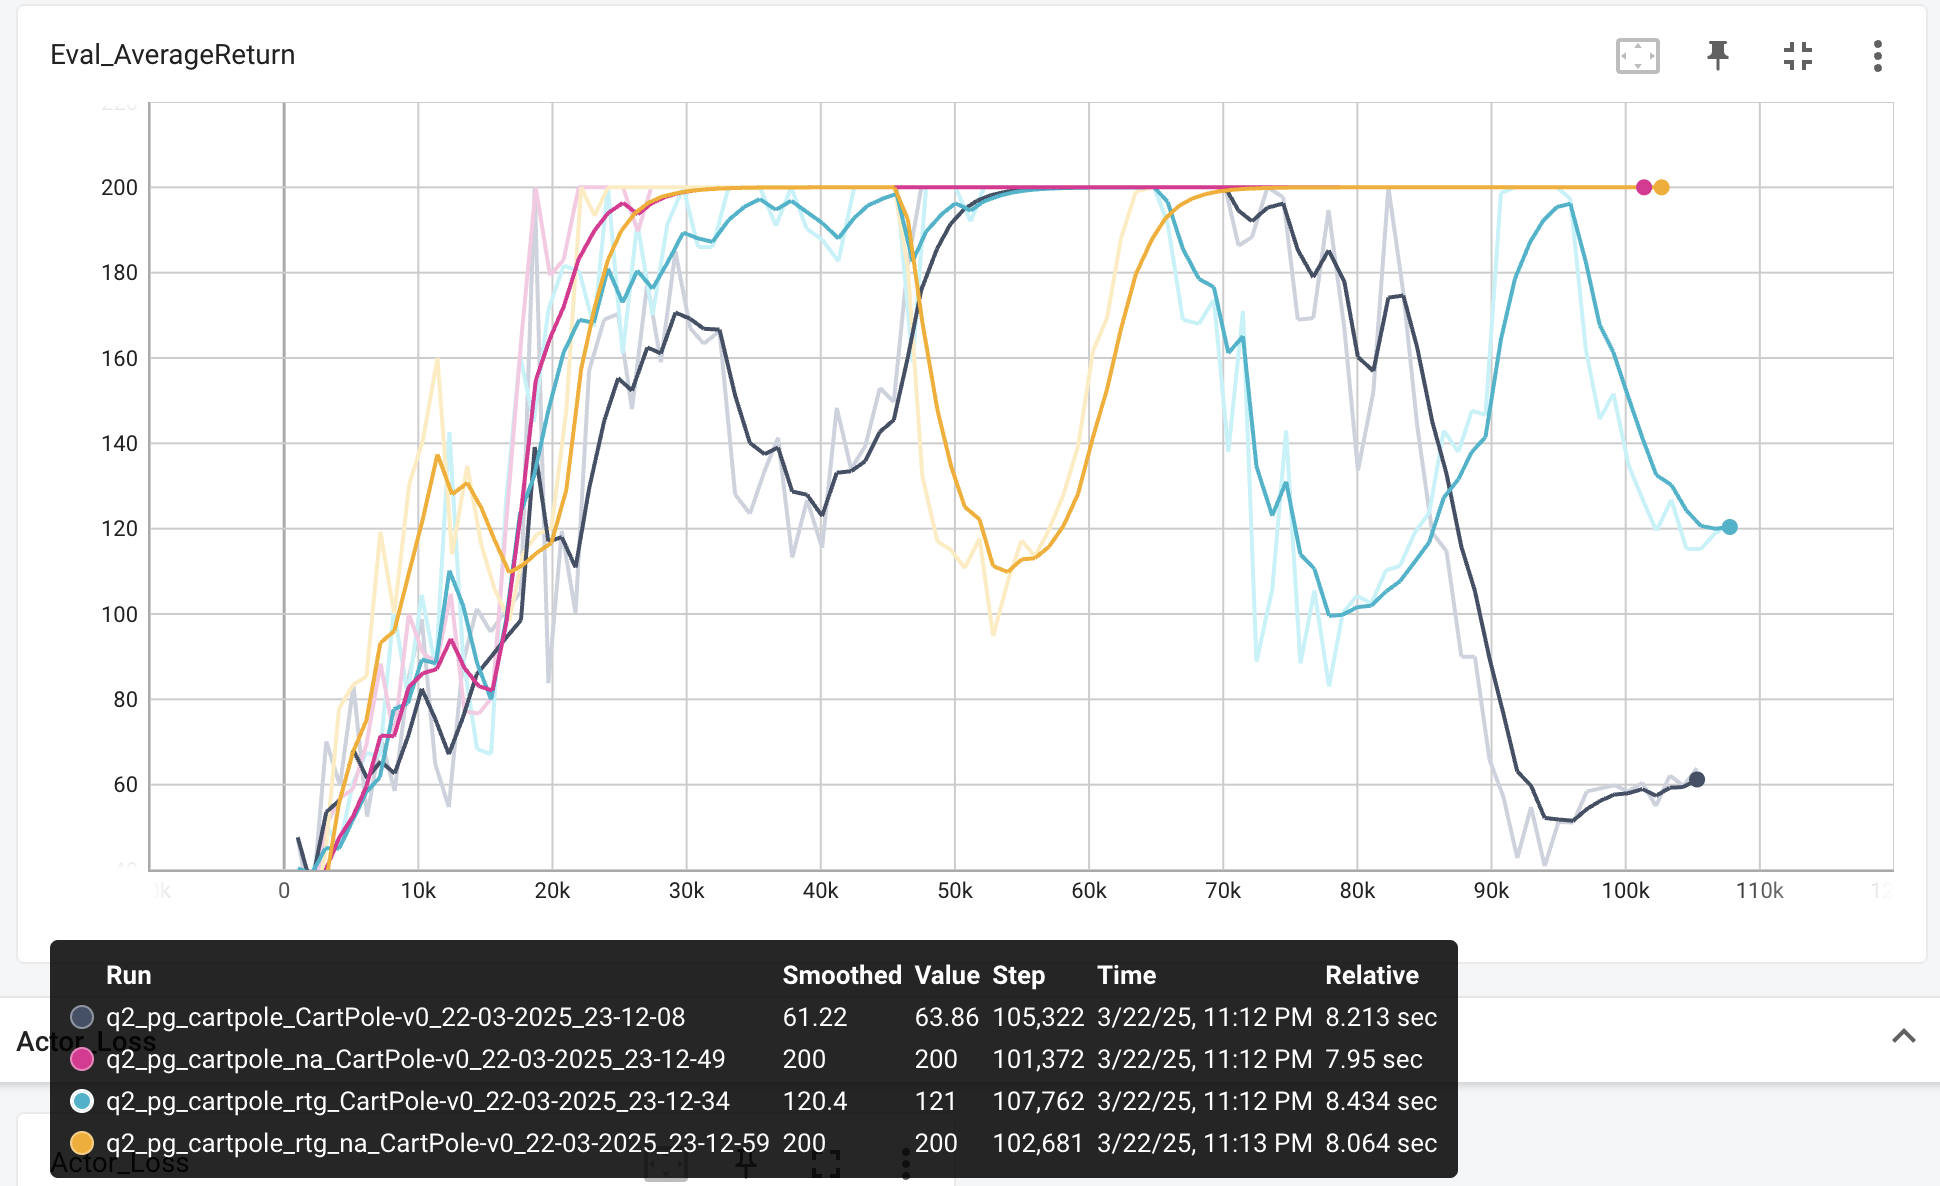
\includegraphics[width=0.5\textwidth]{q3_cartpole_curve.png}
    \caption{Learning curve for small batch cartpole experiments}
    \label{fig:q3_cartpole_curve}
\end{figure}

\begin{figure}[htbp]
    \centering
    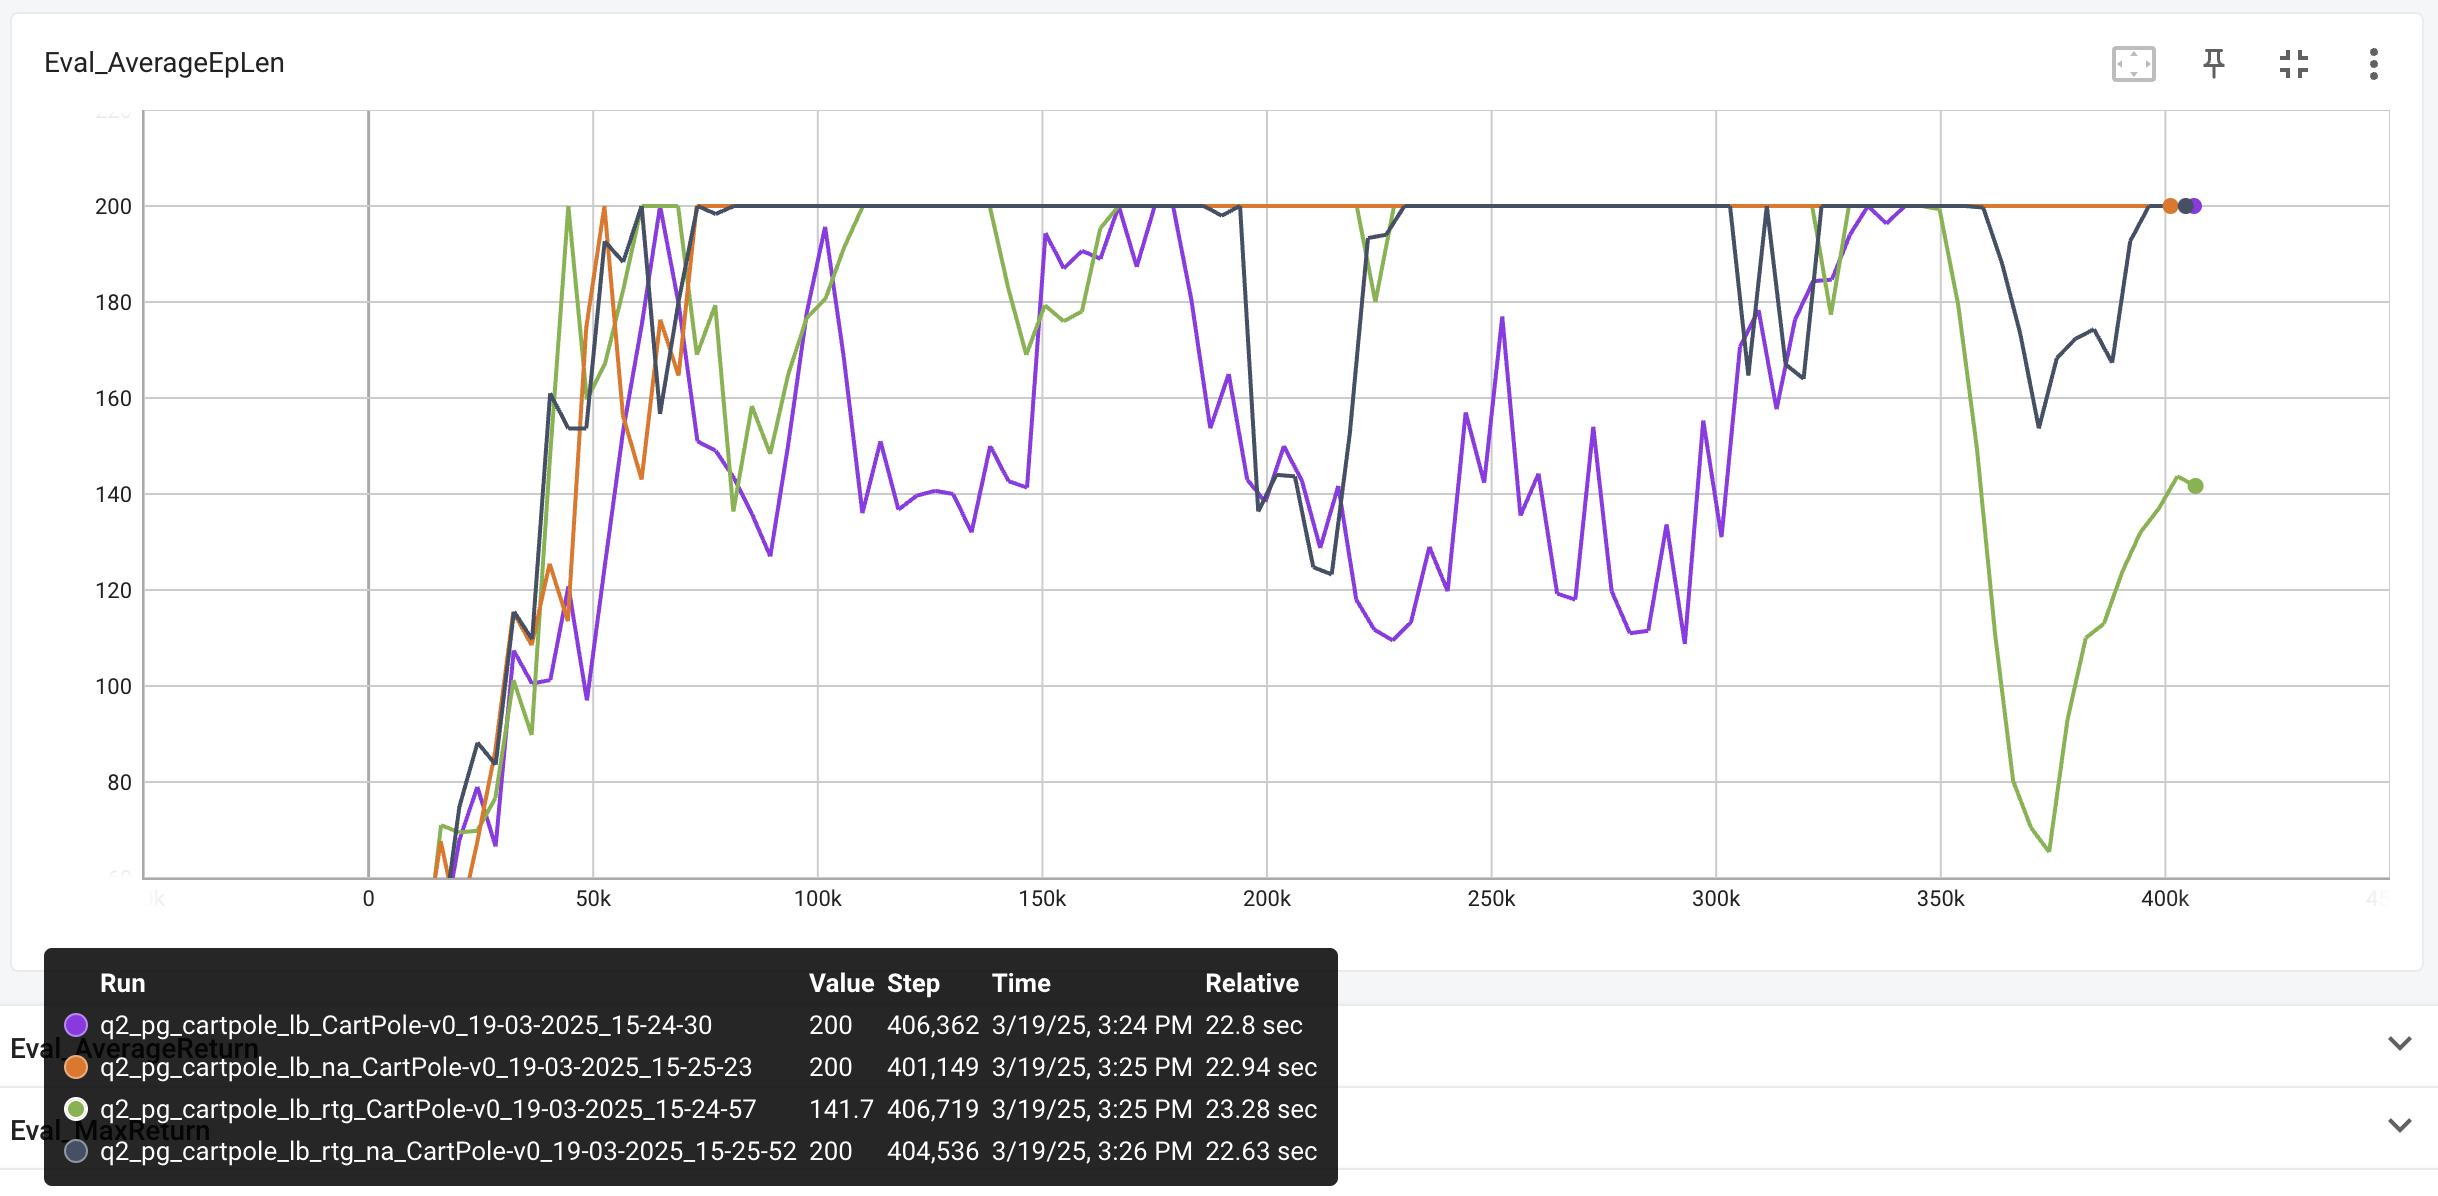
\includegraphics[width=0.5\textwidth]{q3_cartpole_lb_curve.png}
    \caption{Learning curve for large batch cartpole experiments}
    \label{fig:q3_cartpole_lb_curve}
\end{figure}

\item Answer the following questions briefly: 
\begin{itemize}
\item Which value estimator has better performance without advantage normalization: the trajectory-centric one, or the one using reward-to-go?
\begin{itemize}
    \item The one using reward-to-go
\end{itemize}
\item Did advantage normalization help?
\begin{itemize}
    \item Yes, all variants (trajectory centric v.s. reward-to-go, small v.s. large batch) benefited when advantage normalization is used.
\end{itemize}
\item Did the batch size make an impact?
\begin{itemize}
    \item Yes, training was more stable with a bigger batch size.
\end{itemize}
\end{itemize}
\item Provide the exact command line configurations (or \texttt{\#@params} settings in Colab) you used to run your experiments, including any parameters changed from their defaults.
\begin{itemize}
    \item No parameters were changed. The default command line configuration from the homework specs were used.
\end{itemize}
\end{itemize}

\newpage\section{Neural Network Baseline}
\begin{itemize}
    \item Plot a learning curve for the baseline loss.
\begin{figure}[htbp]
    \centering
    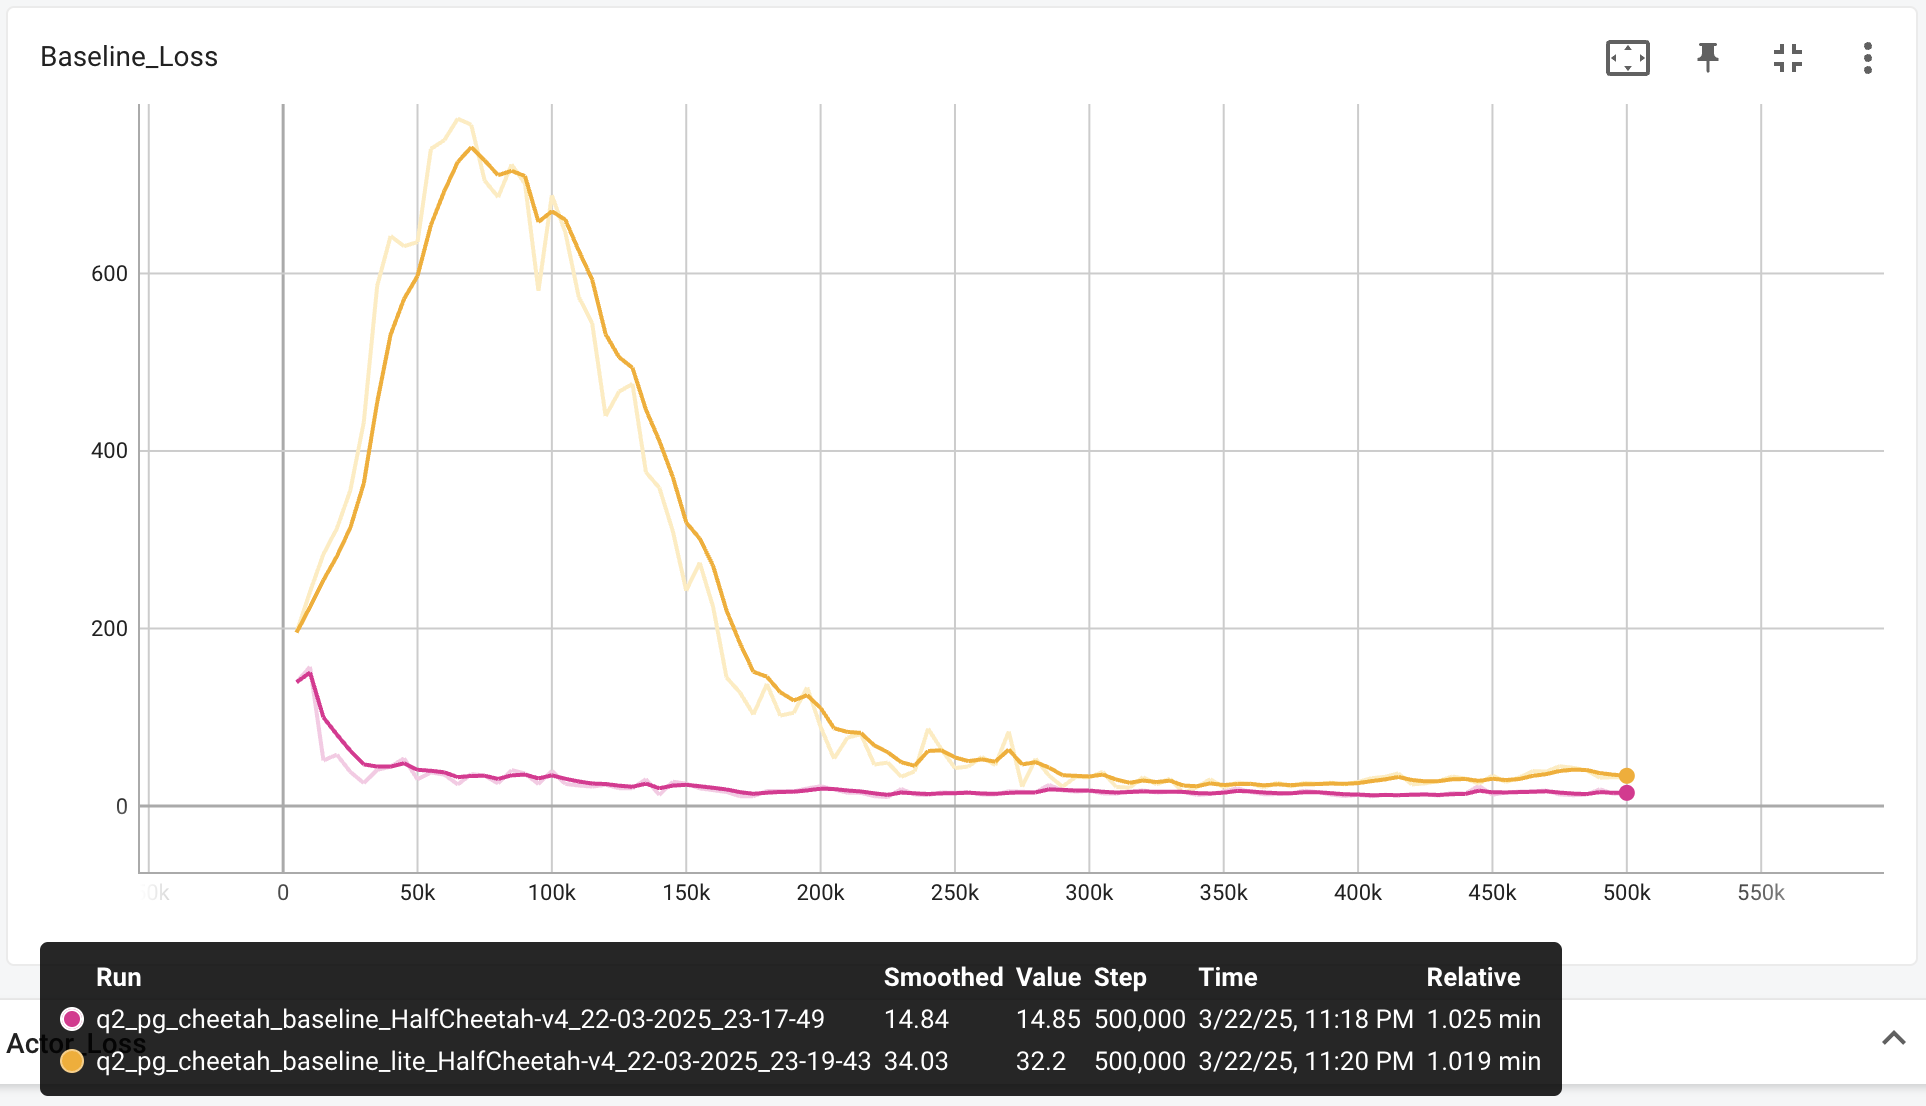
\includegraphics[width=0.5\textwidth]{q4_baseline_loss.png}
    \caption{Learning curves for baseline losses}
    \label{fig:q4_baseline_loss}
\end{figure}
    \item Plot a learning curve for the eval return. You should expect to achieve an average return over 300 for the baselined version.
\begin{figure}[htbp]
    \centering
    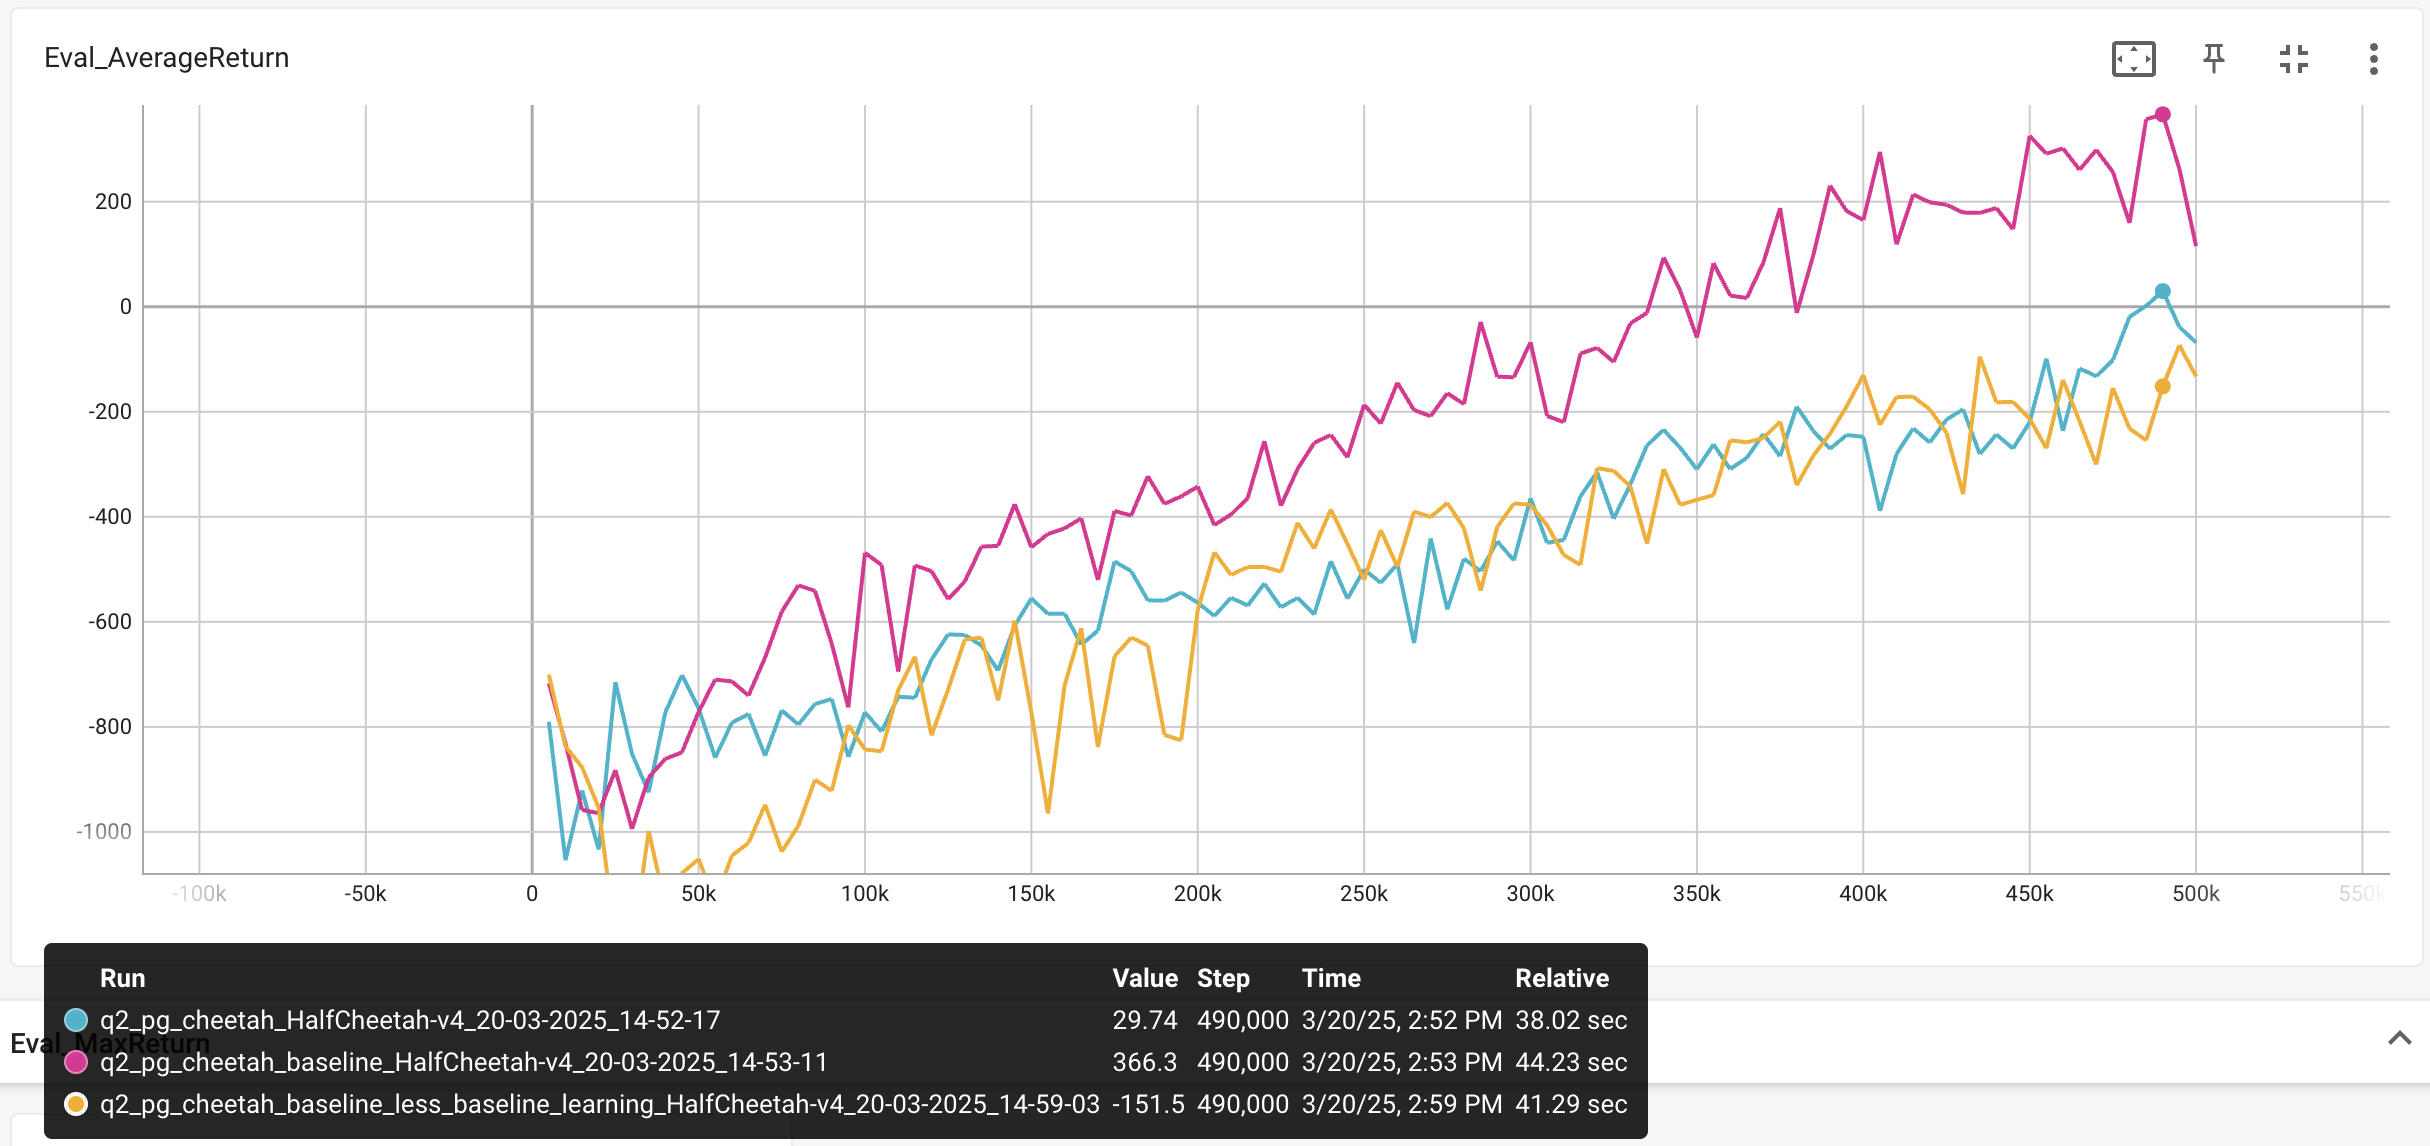
\includegraphics[width=0.5\textwidth]{q4_avg_eval_return.png}
    \caption{Learning curves for average eval returns}
    \label{fig:q4_avg_eval_return}
\end{figure}
    \item Run another experiment with a decreased number of baseline gradient steps (\verb|-bgs|) and/or baseline learning rate (\verb|-blr|). How does this affect (a) the baseline learning curve and (b) the performance of the policy?
\begin{enumerate}[label=(\alph*)]
    \item The baseline loss shot up initially and stabilized at about 2.5x of original setting.
    \item Performance was even worse than the experiment without baseline initially, and eventually they roughly match.
    \item Experiment setup: lr=1e-3 (v.s. original 1e-2) and bgs=2 (v.s. original 5)
\end{enumerate}
    \item \textbf{Optional:} Add \verb|-na| back to see how much it improves things. Also, set \verb|video_log_freq 10|, then open TensorBoard and go to the ``Images'' tab to see some videos of your HalfCheetah walking along!
\end{itemize}

\newpage\section{Generalized Advantage Estimation}
\begin{itemize}
    \item Provide a single plot with the learning curves for the \verb|LunarLander-v2| experiments that you tried. Describe in words how $\lambda$ affected task performance. The run with the best performance should achieve an average score close to 200 (180+).
    \begin{itemize}
    \item For $\lambda \in \{0, 0.95\}$, performance improved initially to be able to achieve positive returns, but regressed as learning continued. This is likely due to the high bias of the gradient estimates.
    \item For $\lambda \in \{0.99, 1\}$, performance kept improving and eventually the returns flatten out at above 100. This seems to suggest that although higher $\lambda$ values lead to higher variance, the reduction in bias outweighs the increase in variance and ultimately leads to better performance.
    \item $\lambda = 0.98$ strikes the best balance between bias/variance and achieves the best peak performance (although less stable than higher $\lambda$ values).
\end{itemize}
\begin{figure}[htbp]
    \centering
    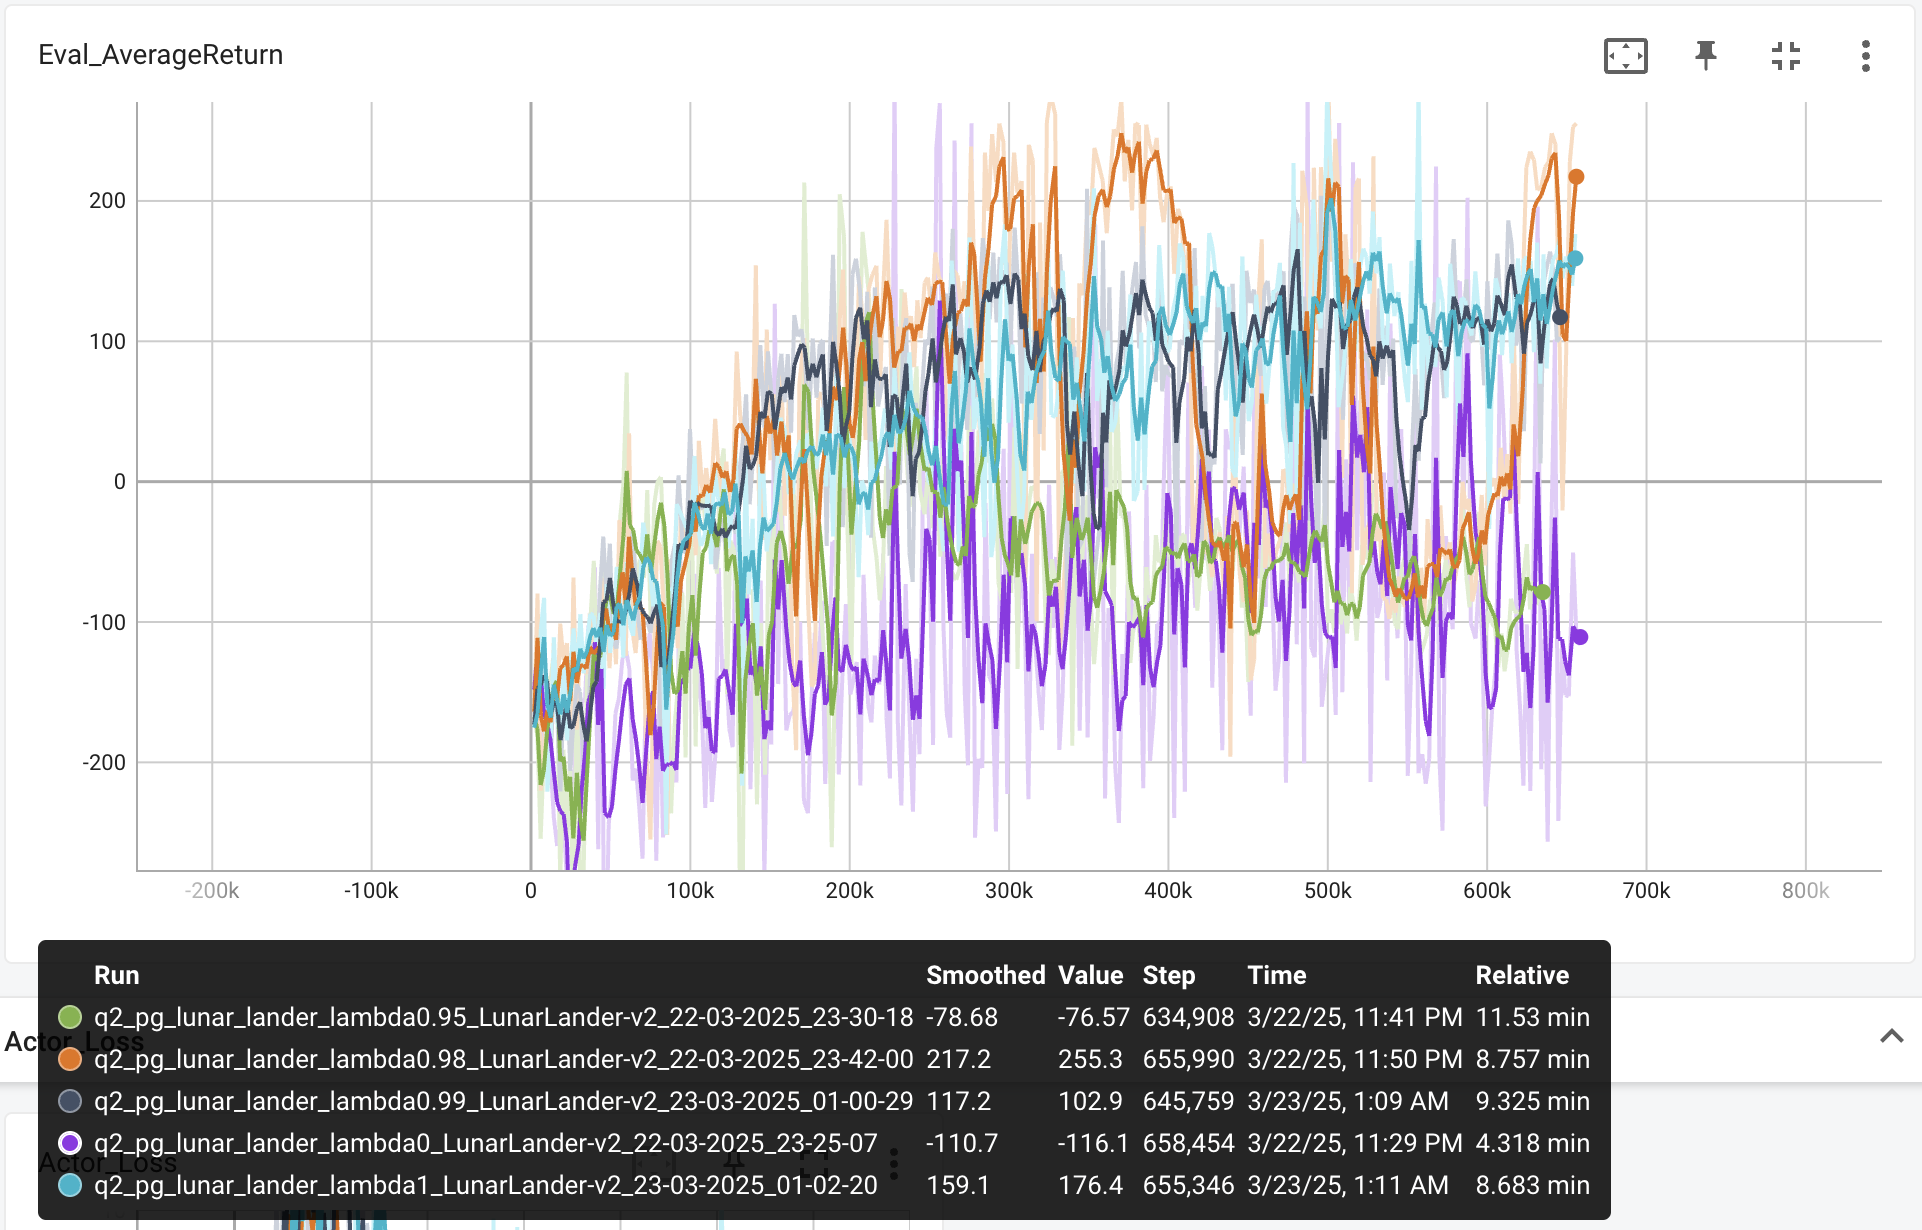
\includegraphics[width=0.5\textwidth]{q5_avg_eval_return.png}
    \caption{Learning curves for various $\lambda$ values}
    \label{fig:q5_avg_eval_return}
\end{figure}
    \item Consider the parameter $\lambda$. What does $\lambda = 0$ correspond to? What about $\lambda = 1$? Relate this to the task performance in \verb|LunarLander-v2| in one or two sentences.
\begin{itemize}
    \item $\lambda = 0$ corresponds to 1-step Monte Carlo estimate (bootstrapping) of $A^\pi(s_t, a_t)$, whereas $\lambda=1$ corresponds to full Monte Carlo estimate.
    \item Lower $\lambda$ values $(0, 0.95)$ lead to higher bias lower variance, whereas higher $\lambda$ values $(0.99, 1)$ lead to lower bias and higher variance. In this particular setup, it seemns to matter more to have lower bias than lower variance. $\lambda=0.98$ is the best tradeoff and achieves the best performance.
\end{itemize}
\end{itemize}

\newpage\section{Hyperparameter Tuning}
\begin{enumerate}
    \item Provide a set of hyperparameters that achieve high return on \verb|InvertedPendulum-v4| in as few environment steps as possible.
    \begin{verbatim}
    for seed in $(seq 1 5); do
        python cs285/scripts/run_hw2.py --env_name InvertedPendulum-v4 -n 100 \
        --exp_name pendulum_best \
        --discount 0.95 -rtg --use_baseline -na --gae_lambda 0.98 \
        --batch_size 200 -l 3 -blr 1e-4 -bgs 1000 \
        --seed $seed
    done
    \end{verbatim}
    \item Show learning curves for the average returns with your hyperparameters and with the default settings, with environment steps on the $x$-axis. Returns should be averaged over 5 seeds.
    \begin{figure}[htbp]
        \centering
        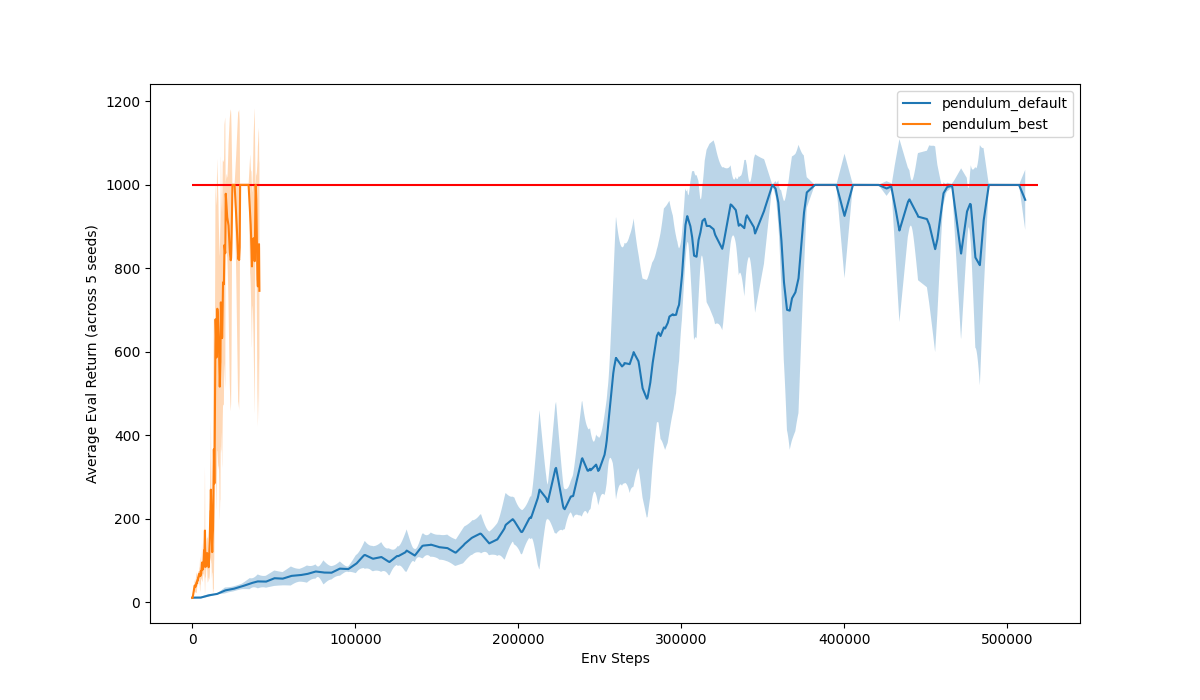
\includegraphics[width=0.5\textwidth]{q6_curves.png}
        \caption{Learning curves for the best performing hyperparameters v.s. default}
        \label{fig:q6_curves}
    \end{figure}
\end{enumerate}

\newpage\section{(Extra Credit) Humanoid}
\begin{enumerate}
    \item Plot a learning curve for the Humanoid-v4 environment. You should expect to achieve an average return of at least 600 by the end of training. Discuss what changes, if any, you made to complete this problem (for example: optimizations to the original code, hyperparameter changes, algorithmic changes).
\end{enumerate}
\begin{figure}[htbp]
    \centering
    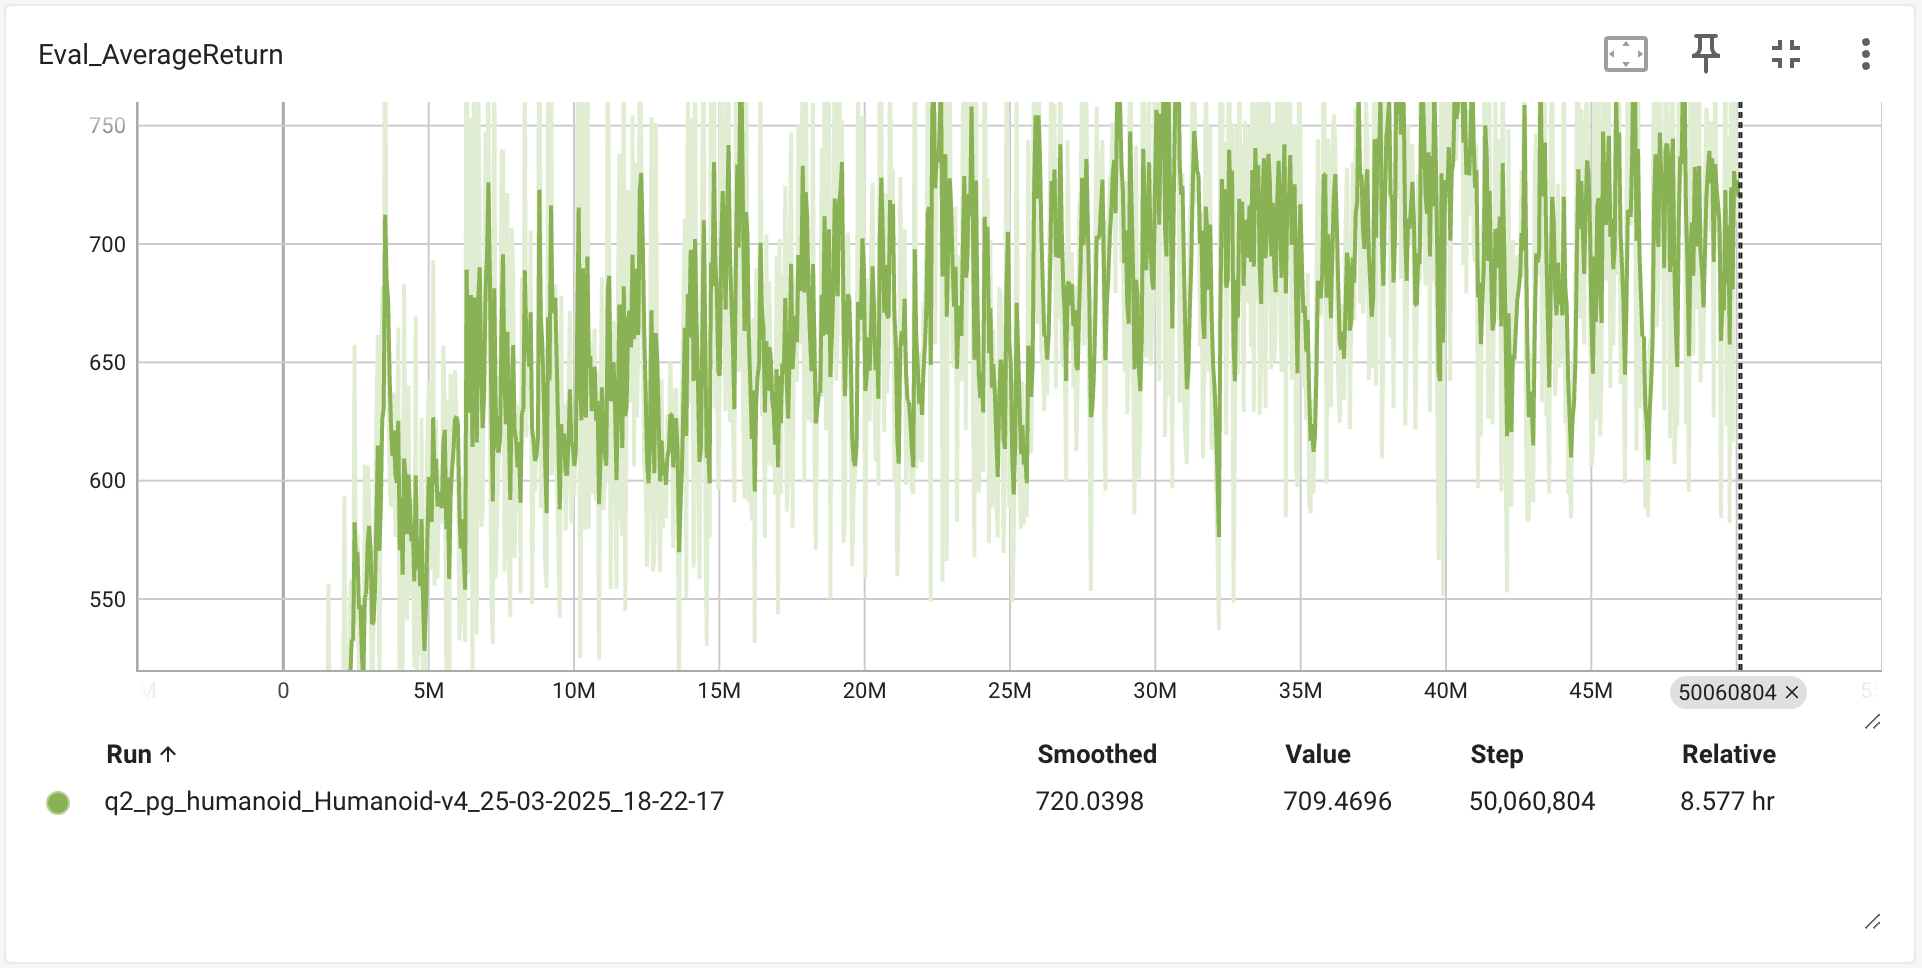
\includegraphics[width=0.5\textwidth]{q7_avg_eval_return.png}
    \caption{Learning curves for Humanoid}
    \label{fig:q7_avg_eval_return}
\end{figure}

\newpage\section{Analysis}
\label{sec:analysis}
Consider the following infinite-horizon MDP:
% https://q.uiver.app/#q=WzAsMixbMCwwLCJzIl0sWzAsMSwic19GIl0sWzAsMSwiYV8yIl1d
\[\begin{tikzcd}
	s_1 & {s_F}
	\arrow["{a_2}", from=1-1, to=1-2]
    \arrow["{a_1}", loop left, from=1-1, to=1-1]
\end{tikzcd}\]
\newcommand{\Rmax}[0]{R_{\textrm{max}}}
\newcommand{\E}[0]{\mathbb{E}}
\newcommand{\var}[0]{\textrm{Var}}
\crefname{question}{part}{parts}
\Crefname{question}{Part}{Parts}
\newcommand\question[1][]{\item\refstepcounter{subsection}\label[question]{#1}}

At each step, the agent stays in state $s_1$ and receives reward 1 if it takes action $a_1$, and receives reward 0 and terminates the episode otherwise.
Parametrize the policy as stationary (not dependent on time) with a single parameter:
\[\pi_\theta(a_1|s_1) = \theta, \pi_\theta(a_2|s_1) = 1-\theta\]

\begin{enumerate}
\question[sec:analysis1] Applying policy gradients
\begin{enumerate}
    \item Use policy gradients to compute the gradient of the expected return $R(\tau)$ with respect to the parameter $\theta$. \textbf{Do not use discounting.}

    \textbf{Hint}: to compute $\sum_{k=1}^\infty k\alpha^{k-1}$, you can write:
    \[\sum_{k=1}^\infty k\alpha^{k-1} = \sum_{k=1}^\infty \frac{d}{d\alpha}\alpha^k = \frac{d}{d\alpha}\sum_{k=1}^\infty\alpha^k\]

\textbf{Solution:} For any $k >= 0$, let $\tau_k$ denote the trajectory where the agent takes action $a_1$ $k$ times before taking an action $a_2$ that terminates the trajectory. Note that $\tau_k$ has the following properties.
\begin{enumerate}
    \item $p_\theta(\tau_k) = \theta^k(1-\theta)$
    \item $r(\tau_k) = k$
    \item $\nabla_\theta \log p_\theta(\tau_k) = \sum_{t=1}^k \nabla_\theta \log \pi_\theta(a_1 | s_1) + \nabla_\theta \log \pi_\theta(a_2 | s_1) = \frac{k}{\theta} - \frac{1}{1 - \theta}$
\end{enumerate}

Therefore, we can derive the policy gradient as follows.

\begin{align}
\nabla_\theta J(\theta) &= \mathbb{E}_{\tau \sim p_\theta(\tau)}[\nabla_\theta \log p_\theta(\tau) \cdot r(\tau)] \\ 
&= \sum_{k=0}^{\infty} p_\theta(\tau_k) \cdot \nabla_\theta \log p_\theta(\tau_k) \cdot r(\tau_k) \\
&= \sum_{k=0}^{\infty} \theta^k(1-\theta) \cdot (\frac{k}{\theta} - \frac{1}{1 - \theta}) \cdot k \\
&= \sum_{k=0}^{\infty} \theta^k(1-\theta) \cdot \frac{k - (k+1)\theta}{\theta(1-\theta)} \cdot k \\
&= \sum_{k=0}^{\infty} k^2\theta^{k-1} - k(k+1)\theta^k \\
&= \sum_{k=0}^{\infty} k^2\theta^{k-1} - (k+1)^2\theta^k + (k+1)\theta^k \\
&= \sum_{k=0}^{\infty} k^2\theta^{k-1} - \sum_{k=0}^{\infty}(k+1)^2\theta^k + \sum_{k=0}^{\infty}(k+1)\theta^k \\
&= \sum_{k=1}^{\infty} k^2\theta^{k-1} - \sum_{k=1}^{\infty} k^2\theta^{k-1} + \sum_{k=1}^{\infty}k\theta^{k-1} \\
&= \frac{d}{d\theta}\sum_{k=1}^{\infty}\theta^k = \frac{d}{d\theta}\frac{\theta}{1-\theta} = \frac{1}{(1-\theta)^2}
\end{align}

    \item \label{exact_gradient} Compute the expected return of the policy $\E_{\tau \sim \pi_\theta} R(\tau)$ directly. Compute the gradient of this expression with respect to $\theta$ and verify that this matches the policy gradient.

\textbf{Solution:}
Note that under the policy $\pi_\theta$, the reward $r(\tau_k)$ follows a geometric distribution with success probability $1 - \theta$, so 

\[J(\theta) = \mathbb{E}[r(\tau_k)] = \frac{\theta}{1 - \theta}\]

Therefore, we have
\[\nabla_\theta J(\theta) = \frac{d}{d\theta} \frac{\theta}{1 - \theta} = \frac{1}{(1-\theta)^2} \]

\end{enumerate}
\newpage
\question[sec:analysis2] Compute the variance of the policy gradient in closed form and describe the properties of the variance with respect to $\theta$. For what value(s) of $\theta$ is variance minimal? Maximal? (Once you have an exact expression for the variance you can eyeball the min/max).

\textbf{Hint:}  Once you have it expressed as a sum of terms $P(\theta)/Q(\theta)$ where $P$ and $Q$ are polynomials, you can use a symbolic computing program (Mathematica, SymPy, etc) to simplify to a single rational expression.

\textbf{Solution:}

Given 
\[\text{VAR}_{\tau \sim p_\theta(\tau)}[\nabla_\theta \log p_\theta(\tau) r(\tau)] = \mathbb{E}_{\tau \sim p_\theta(\tau)}[(\nabla_\theta \log p_\theta(\tau) r(\tau))^2] - (\mathbb{E}_{\tau \sim p_\theta(\tau)}[\nabla_\theta \log p_\theta(\tau) r(\tau)])^2\]

and we know that 

\[(\mathbb{E}_{\tau \sim p_\theta(\tau)}[\nabla_\theta \log p_\theta(\tau) r(\tau)])^2 = (\frac{1}{(1 - \theta)^2})^2 = \frac{1}{(1 - \theta)^4}\]

we focus on computing $\mathbb{E}_{\tau \sim p_\theta(\tau)}[(\nabla_\theta \log p_\theta(\tau) r(\tau))^2]$ first.

\begin{align}
&\mathbb{E}_{\tau \sim p_\theta(\tau)}[(\nabla_\theta \log p_\theta(\tau) r(\tau))^2] \\
=& \sum_{k=0}^{\infty} p_\theta(\tau_k)(\nabla_\theta \log p_\theta(\tau) r(\tau))^2 \\
=& \sum_{k=0}^{\infty}\theta^k(1-\theta)((\frac{k}{\theta} - \frac{1}{1-\theta})k)^2 \\
=& \sum_{k=0}^{\infty}\theta^k(1-\theta)(\frac{k^4}{\theta^2} - \frac{2k^3}{\theta(1-\theta)} + \frac{k^2}{(1-\theta)^2}) \\
=& \frac{1-\theta}{\theta^2}\sum_{k=0}^{\infty}k^4\theta^k - \frac{2}{\theta}\sum_{k=0}^{\infty}k^3\theta^k + \frac{1}{1-\theta}\sum_{k=0}^{\infty}k^2\theta^k \\
=& \frac{1-\theta}{\theta^2}\cdot\frac{\theta(1 + 11\theta + 11\theta^2 + \theta^3)}{(1-\theta)^5} - \frac{2}{\theta}\cdot\frac{\theta(1 + 4\theta + \theta^2)}{(1-\theta)^4} + \frac{1}{1-\theta}\cdot\frac{\theta(1+\theta)}{(1-\theta)^3} \\
=& \frac{1 + 11\theta + 11\theta^2 + \theta^3}{\theta(1-\theta)^4} - \frac{2\theta(1 + 4\theta + \theta^2)}{\theta(1-\theta)^4} + \frac{\theta^2(1+\theta)}{\theta(1-\theta)^4} \\
=& \frac{4\theta^2 + 9\theta +1}{\theta(1-\theta)^4}
\end{align}

Plugging it back, we get 
\[
\text{VAR}_{\tau \sim p_\theta(\tau)}[\nabla_\theta \log p_\theta(\tau) r(\tau)] = \frac{4\theta^2 + 9\theta +1}{\theta(1-\theta)^4} - \frac{1}{(1 - \theta)^4} = \frac{4\theta^2 + 8\theta +1}{\theta(1-\theta)^4}
\]

\newpage
\question[sec:analysis3] Apply return-to-go as an advantage estimator.
\begin{enumerate}
    \item Write the modified policy gradient and confirm that it is unbiased.

\textbf{Solution:}
\begin{align}
\nabla_{\theta}J(\theta) &= \mathbb{E}_{\tau \sim p_\theta}[\sum_{t=1}^{T}\nabla_\theta \log \pi_\theta(a_t | s_t)(\sum_{t'=t}^{T}r(s_t, a_t))] \\
&= \sum_{k=0}^{\infty}p_\theta(\tau_k)(\sum_{t=1}^k\nabla_\theta\log\pi_\theta(a_t|s_t)(\sum_{t'=t}^{T}r(s_t, a_t)) + \nabla_\theta\log\pi_\theta(a_{k+1} | s_{k+1})r(s_{k+1}, a_{k+1})) \\
&= \sum_{k=0}^{\infty}\theta^k(1-\theta)\sum_{t=1}^{k}\frac{1}{\theta}(k - t + 1) \\
&= \sum_{k=0}^{\infty}\theta^{k-1}(1-\theta)\frac{k(k+1)}{2} \\
&= \frac{1}{2\theta}(\sum_{k=0}^{\infty}k^2\theta^k(1-\theta) + \sum_{k=0}^{\infty}k\theta^k(1-\theta))
\end{align}

Note that the terms in the parentheses are the second and first moments of a geometric distribution, so we have

\[
\sum_{k=0}^{\infty}k^2\theta^k(1-\theta) = \frac{\theta + \theta^2}{(1-\theta)^2}
\]

and
\[
\sum_{k=0}^{\infty}k\theta^k(1-\theta) = \frac{\theta}{1-\theta}
\]

Plugging them back in, we get
\begin{align}
\nabla_{\theta}J(\theta) &= \frac{1}{2\theta}(\sum_{k=0}^{\infty}k^2\theta^k(1-\theta) + \sum_{k=0}^{\infty}k\theta^k(1-\theta)) \\
&= \frac{1}{2\theta}(\frac{\theta + \theta^2}{(1-\theta)^2} + \frac{\theta}{1-\theta}) \\
&= \frac{1}{(1-\theta)^2}
\end{align}

    \item Compute the variance of the return-to-go policy gradient and plot it on $[0, 1]$ alongside the variance of the original estimator.

\textbf{Solution:}

\begin{align}
&\mathbb{E}_{\tau \sim p_\theta}[(\sum_{t=1}^{T}\nabla_\theta \log \pi_\theta(a_t | s_t)(\sum_{t'=t}^{T}r(s_t, a_t)))^2] \\
=& \sum_{k=0}^{\infty}\theta^k(1-\theta)(\sum_{t=1}^{k}\frac{1}{\theta}(k - t + 1))^2 \\
=& \sum_{k=0}^{\infty}\theta^{k-2}(1-\theta)(\sum_{t=1}^{k}k - t + 1)^2 \\
=& \sum_{k=0}^{\infty}\theta^{k-2}(1-\theta)\frac{k^2(k+1)^2}{4} \\
=& \sum_{k=0}^{\infty}\theta^{k-2}(1-\theta)\frac{k^4+2k^3+k^2}{4} \\
=& \frac{1-\theta}{4\theta^2}(\sum_{k=0}^{\infty}k^4\theta^k + 2\sum_{k=0}^{\infty}k^3\theta^k + \sum_{k=0}^{\infty}k^4\theta^k) \\
=& \frac{1-\theta}{4\theta^2}(\frac{\theta(1 + 11\theta + 11\theta^2 + \theta^3)}{(1-\theta)^5} + \frac{2\theta(1 + 4\theta + \theta^2)}{(1-\theta)^4} + \frac{\theta(1+\theta)}{(1-\theta)^3}) \\
=& \frac{\theta^2 + 4\theta + 1}{\theta(1-\theta)^4}
\end{align}

Therefore, we have
\[
\text{VAR}_{\tau \sim p_\theta(\tau)}[\sum_{t=1}^{T}\nabla_\theta \log \pi_\theta(a_t | s_t)(\sum_{t'=t}^{T}r(s_t, a_t))] = \frac{\theta^2 + 4\theta + 1}{\theta(1-\theta)^4} - \frac{1}{(1-\theta)^4} = \frac{\theta^2 + 3\theta + 1}{\theta(1-\theta)^4}
\]

\begin{figure}[htbp]
    \centering
    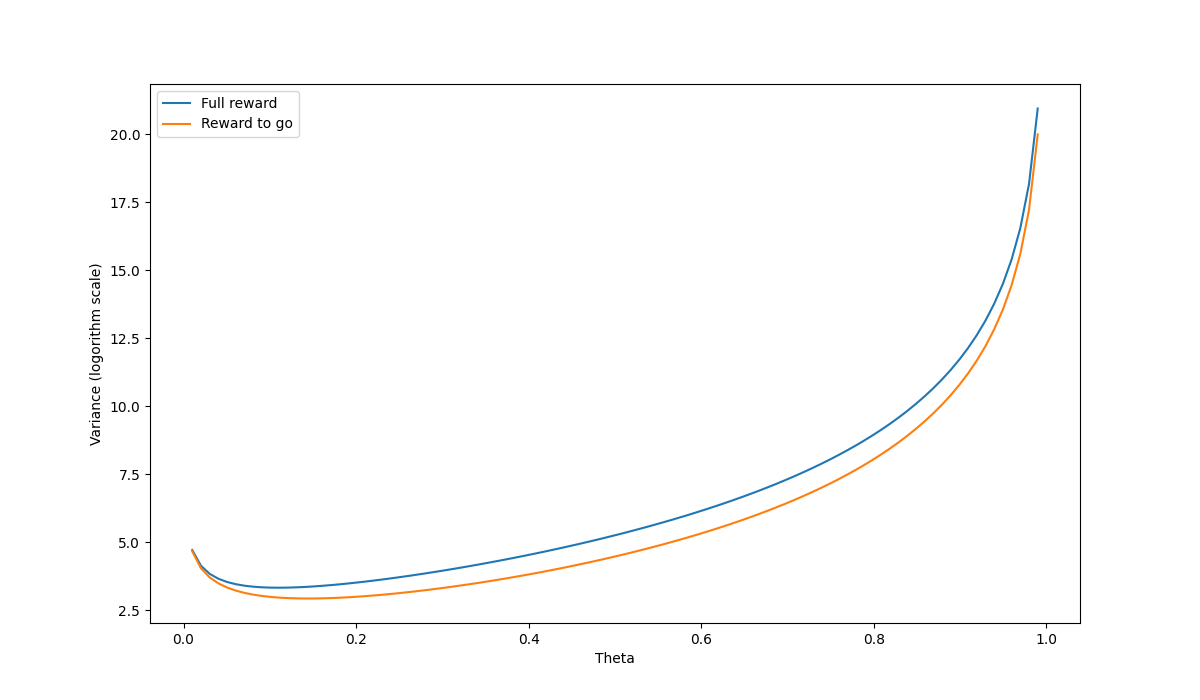
\includegraphics[width=0.5\textwidth]{q8_varience_curves.png}
    \caption{Learning curve for small batch cartpole experiments}
    \label{fig:q8_variance_curves}
\end{figure}

\end{enumerate}
\newpage
\question[sec:analysis4] Consider a finite-horizon $H$-step MDP with sparse reward:
% https://q.uiver.app/#q=WzAsNixbMCwwLCJzXzEiXSxbMSwwLCJzXzIiXSxbMiwwLCJzXzMiXSxbMiwxLCJzX0YiXSxbMywwLCJcXGRvdHMiXSxbNCwwLCJzX0giXSxbMCwxLCJhXzEiXSxbMSwyLCJhXzEiXSxbMCwzLCJhXzIiLDJdLFsyLDQsImFfMSJdLFs0LDVdLFsxLDMsImFfMiJdLFsyLDMsImFfMiIsMV0sWzQsMywiYV8yIiwxXV0=
\[\begin{tikzcd}
	{s_1} & {s_2} & {s_3} & \dots & {s_H} \\
	&& {s_F}
	\arrow["{a_1}", from=1-1, to=1-2]
	\arrow["{a_1}", from=1-2, to=1-3]
	\arrow["{a_2}"', from=1-1, to=2-3]
	\arrow["{a_1}", from=1-3, to=1-4]
	\arrow[from=1-4, to=1-5]
	\arrow["{a_2}", from=1-2, to=2-3]
	\arrow["{a_2}"{description}, from=1-3, to=2-3]
	\arrow["{a_2}"{description}, from=1-4, to=2-3]
\end{tikzcd}\]

The agent receives reward $\Rmax$ if it arrives at $s_H$ and reward $0$ if it arrives at $s_F$ (a terminal state). In other words, the return for a trajectory $\tau$ is given by:
\[R(\tau) = \begin{cases}1 & \tau \textrm{ ends at } s_H \\ 0 & \tau \textrm{ ends at } s_F \end{cases}\]
Using the same policy parametrization as above, consider off-policy policy gradients via importance sampling. Assume we want to compute policy gradients for a policy $\pi_\theta$ with samples drawn from $\pi_{\theta'}$.
\begin{enumerate}
    \item Write the policy gradient with importance sampling.

\textbf{Solution:}
Let $\tau_H$ be the trajectory that ends at $s_H$. We know that $p_\theta(\tau_H) = \theta^{H-1}$, $r(\tau_H)=1$ and $r(\tau) = 0$ for any $\tau \neq \tau_H$.

Assume that we have a sample of trajectories $\tau^{(1)}, \tau^{(2)}, ..., \tau^{(n)}$ drawn from $\pi_{\theta'}$, and let $n_H$ be the number of times $\tau_H$ appear in the sample. The sample policy gradient with importance sampling is the following.

\begin{align}
\nabla_\theta J(\theta) &\approx \frac{1}{n} \sum_{i=1}^{n} \frac{p_\theta(\tau^{(i)})}{p_{\theta'}(\tau^{(i)})} \nabla_\theta \log p_\theta(\tau^{(i)}) r(\tau^{(i)}) \\
&= \frac{n_H}{n}(\frac{\theta}{\theta'})^{H-1}(H-1)\frac{1}{\theta} \\
&= \frac{n_H(H-1)\theta^{H-2}}{n{\theta'}^{H-1}}
\end{align}
    \item Compute its variance.

\textbf{Solution:} To compute the variance of policy gradient with importance sample, we first compute its first and second moments.

\begin{align}
&\mathbb{E}_{\tau \sim p_{\theta'}(\tau)}\left[\frac{p_\theta(\tau)}{p_{\theta'}(\tau)}\nabla_\theta \log p_\theta(\tau) r(\tau)\right] \\
=& p_{\theta'}(\tau_H) \frac{p_\theta(\tau_H)}{p_{\theta'}(\tau_H)}\nabla_\theta \log p_\theta(\tau_H) r(\tau_H)\\
=& p_\theta(\tau_H)\nabla_\theta \log p_\theta(\tau_H) r(\tau_H) \\
=& (H-1)\theta^{H-2}
\end{align}

\begin{align}
&\mathbb{E}_{\tau \sim p_{\theta'}(\tau)}\left[\left(\frac{p_\theta(\tau)}{p_{\theta'}(\tau)}\nabla_\theta \log p_\theta(\tau) r(\tau)\right)^2\right] \\
=& p_{\theta'}(\tau_H) \left(\frac{p_\theta(\tau_H)}{p_{\theta'}(\tau_H)}\nabla_\theta \log p_\theta(\tau_H) r(\tau_H)\right)^2\\
=& (\theta')^{H-1}\left(\left(\frac{\theta}{\theta'}\right)^{H-1}(H-1)\frac{1}{\theta}\right)^2 \\
=& \frac{(H-1)^2\theta^{2H-4}}{{\theta'}^{H-1}}
\end{align}

Combining above, we get 
\[
\text{VAR}_{\tau \sim p_{\theta'}(\tau)}\left[ \frac{p_\theta(\tau)}{p_{\theta'}(\tau)}\nabla_\theta \log p_\theta(\tau) r(\tau)\right] = \frac{(H-1)^2\theta^{2H-4}}{{\theta'}^{H-1}} - (H-1)\theta^{H-2} = \frac{(H-1)\theta^{H-2}}{{\theta'}^{H-1}}\left( (H-1)\theta^{H-2} - {\theta'}^{H-1}\right)
\]

\end{enumerate}

\end{enumerate}

\newpage\section{Survey}
\label{sec:survey}
Please estimate, in minutes, for each problem, how much time you spent (a) writing code and (b) waiting for the results. This will help us calibrate the difficulty for future homeworks. 
\begin{itemize}
    \item \textbf{Policy Gradients:}
    \item \textbf{Neural Network Baseline:}
    \item \textbf{Generalized Advantage Estimation:}
    \item \textbf{Hyperparameters and Sample Efficiency:}
    \item \textbf{Humanoid:}
    \item \textbf{Humanoid:}
    \item \textbf{Analysis -- applying policy gradients:}
    \item \textbf{Analysis -- PG variance:}
    \item \textbf{Analysis -- return-to-go:}
    \item \textbf{Analysis -- importance sampling:}
\end{itemize}

\end{document}
